%!TEX program = lualatex


\documentclass{beamer}
\usetheme[delaunay]{Amurmaple}


\usepackage{tikz}
\usepackage{graphicx}
\usepackage{mathtools}
\usepackage{pgfplots}
\usepackage{graphicx}
\usepackage{subfig}


\usetikzlibrary{arrows.meta, positioning, patterns}

\usepackage{tkz-euclide}


\pgfplotsset{compat=1.17}

\title[CLIPPER]{A Graph-Theoretic Framework for Robust Data Association}
\subtitle{A Summary/Review}
\author{Presented by: Abolfazl Babanazari}
\date{\today}

\begin{document}

\begin{frame}
  \titlepage
\end{frame}

\begin{frame}{Introduction}
  \textbf{Data Association:}
  \begin{itemize}
    \item Objective: To robustly identify a true correspondence between two sets of objects in the presence of noise and outliers.
  \end{itemize}

  \textbf{Mathematical Formulation:}
  \begin{block}{Combinatorial Optimization Problem}
    Given two sets of objects \( \mathcal{A} \) and \( \mathcal{A^\prime} \) and a putative association set \( \mathcal{U} \subseteq \mathcal{A}
    \times \mathcal{A^\prime} \) , find a associations \( \mathcal{U}^\prime \subseteq \mathcal{U} \) minimize error function in a given transformation model.
  \end{block}\
  \onslide<2->{
    \textbf{Challenges:}
    \begin{itemize}
      \item<3-> Computational complexity of combinatorial optimization
      \item<4-> Maintaining high accuracy in high-noise, high-outlier conditions.
    \end{itemize}
  }
\end{frame}


\begin{frame}{Introuduction}
  \vspace{1mm}
  \textbf{Applications in Computer Vision \& Robotics}
  \begin{itemize}
    \item<1-> Point cloud registration
      \only<1>{
        \begin{figure}
          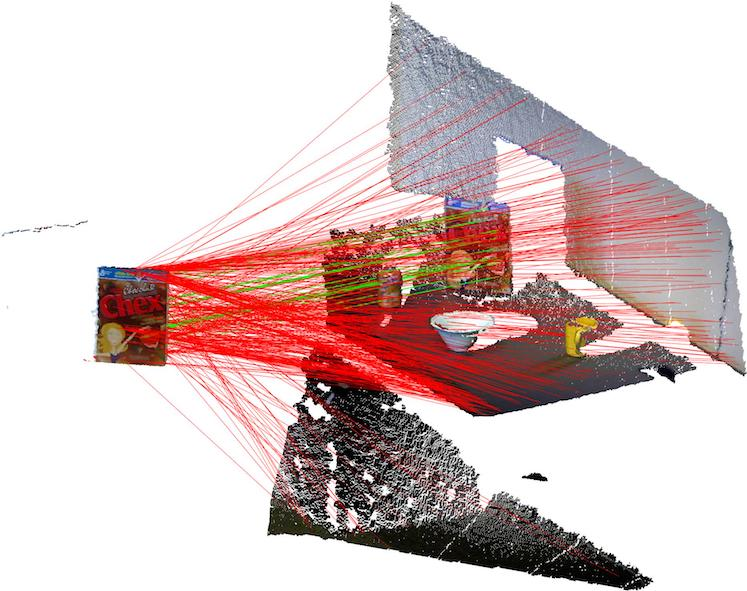
\includegraphics[width=5cm]{images/pointcloud-registration-init.jpg}
          \hspace{5mm}
          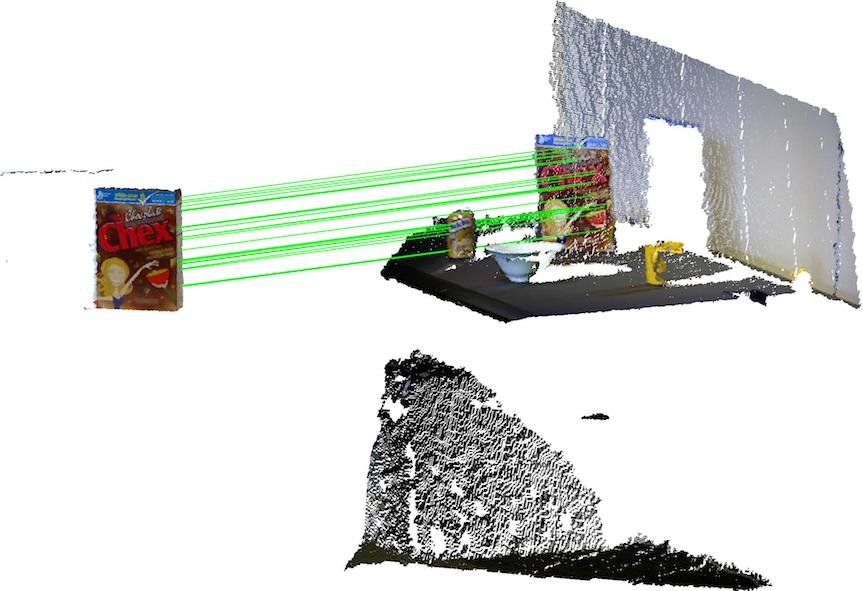
\includegraphics[width=5cm]{images/pointcloud-registration-results.jpg}
        \end{figure}
      }
    \item<2->  Multiple object tracking
      \only<2>{
        \begin{figure}
          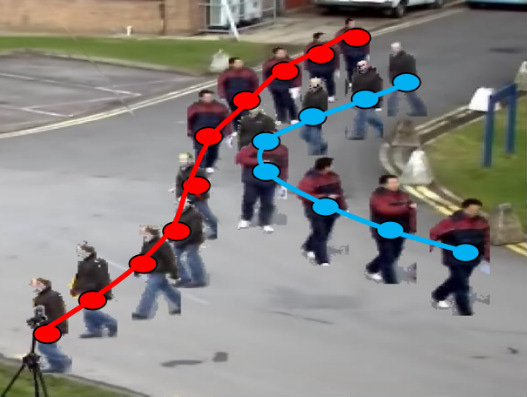
\includegraphics[width=5cm]{images/object-tracking-wrong.jpg}
          \hspace{5mm}
          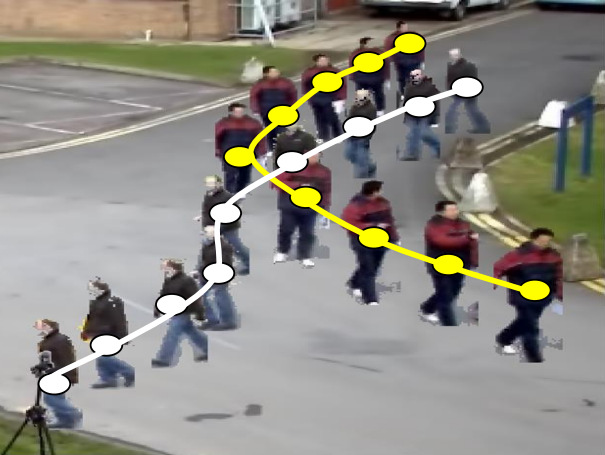
\includegraphics[width=5cm]{images/object-tracking-right.jpg}
        \end{figure}
      }
    \item<3-> Object detection
      \only<3> {
        \begin{figure}
          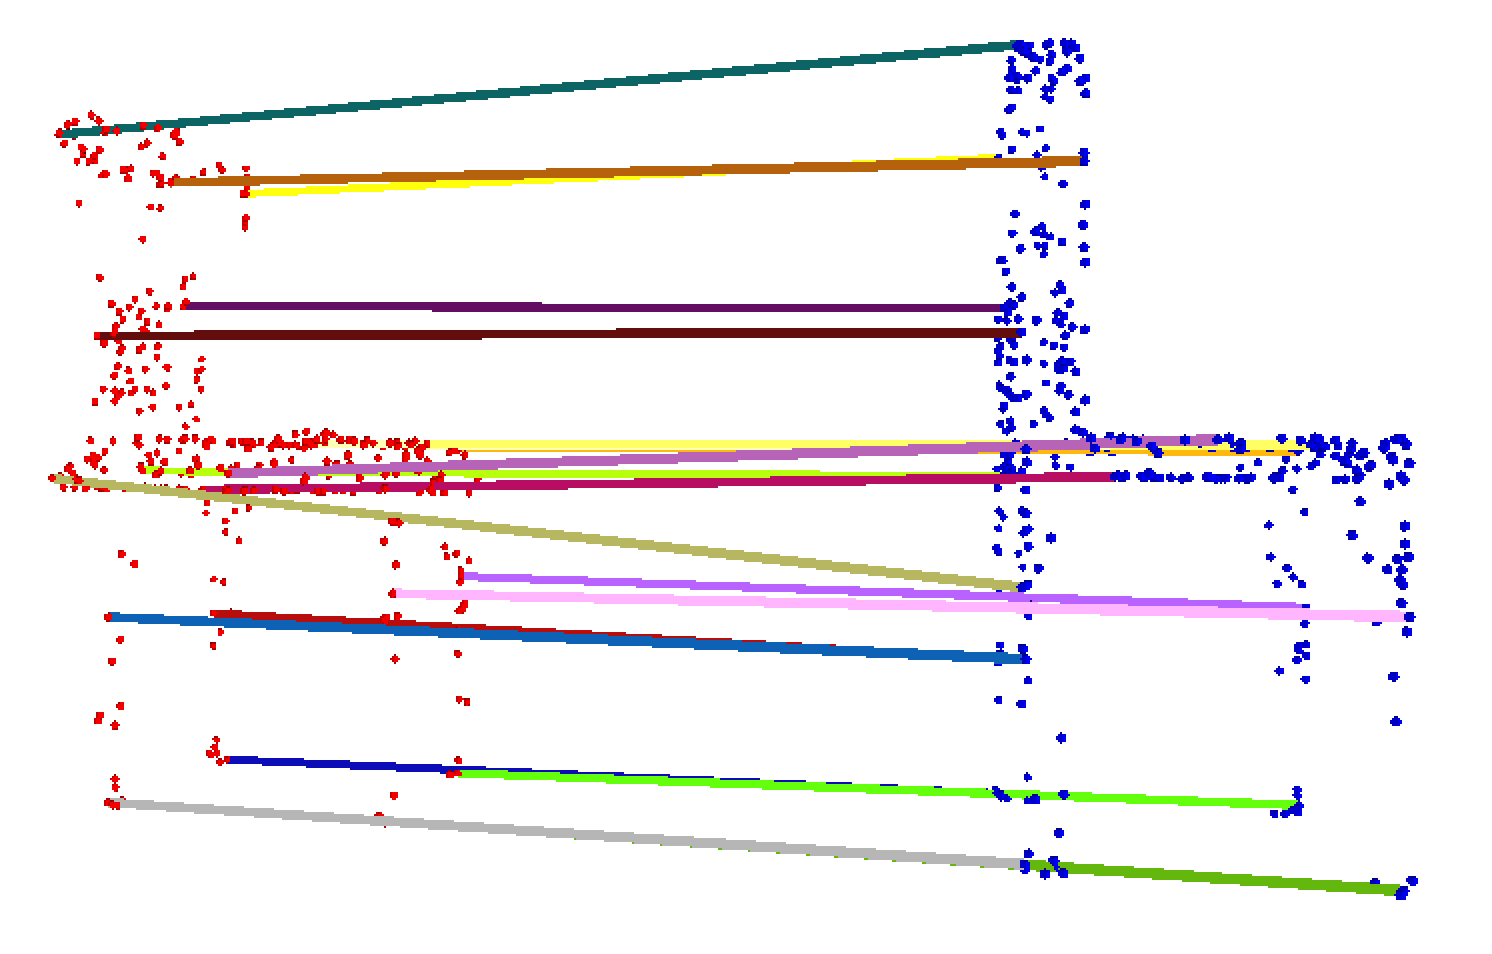
\includegraphics[width=10cm]{images/object-detection.png}
        \end{figure}
      }
    \item<4-> Shape alignment
      \only<4> {
        \begin{figure}
          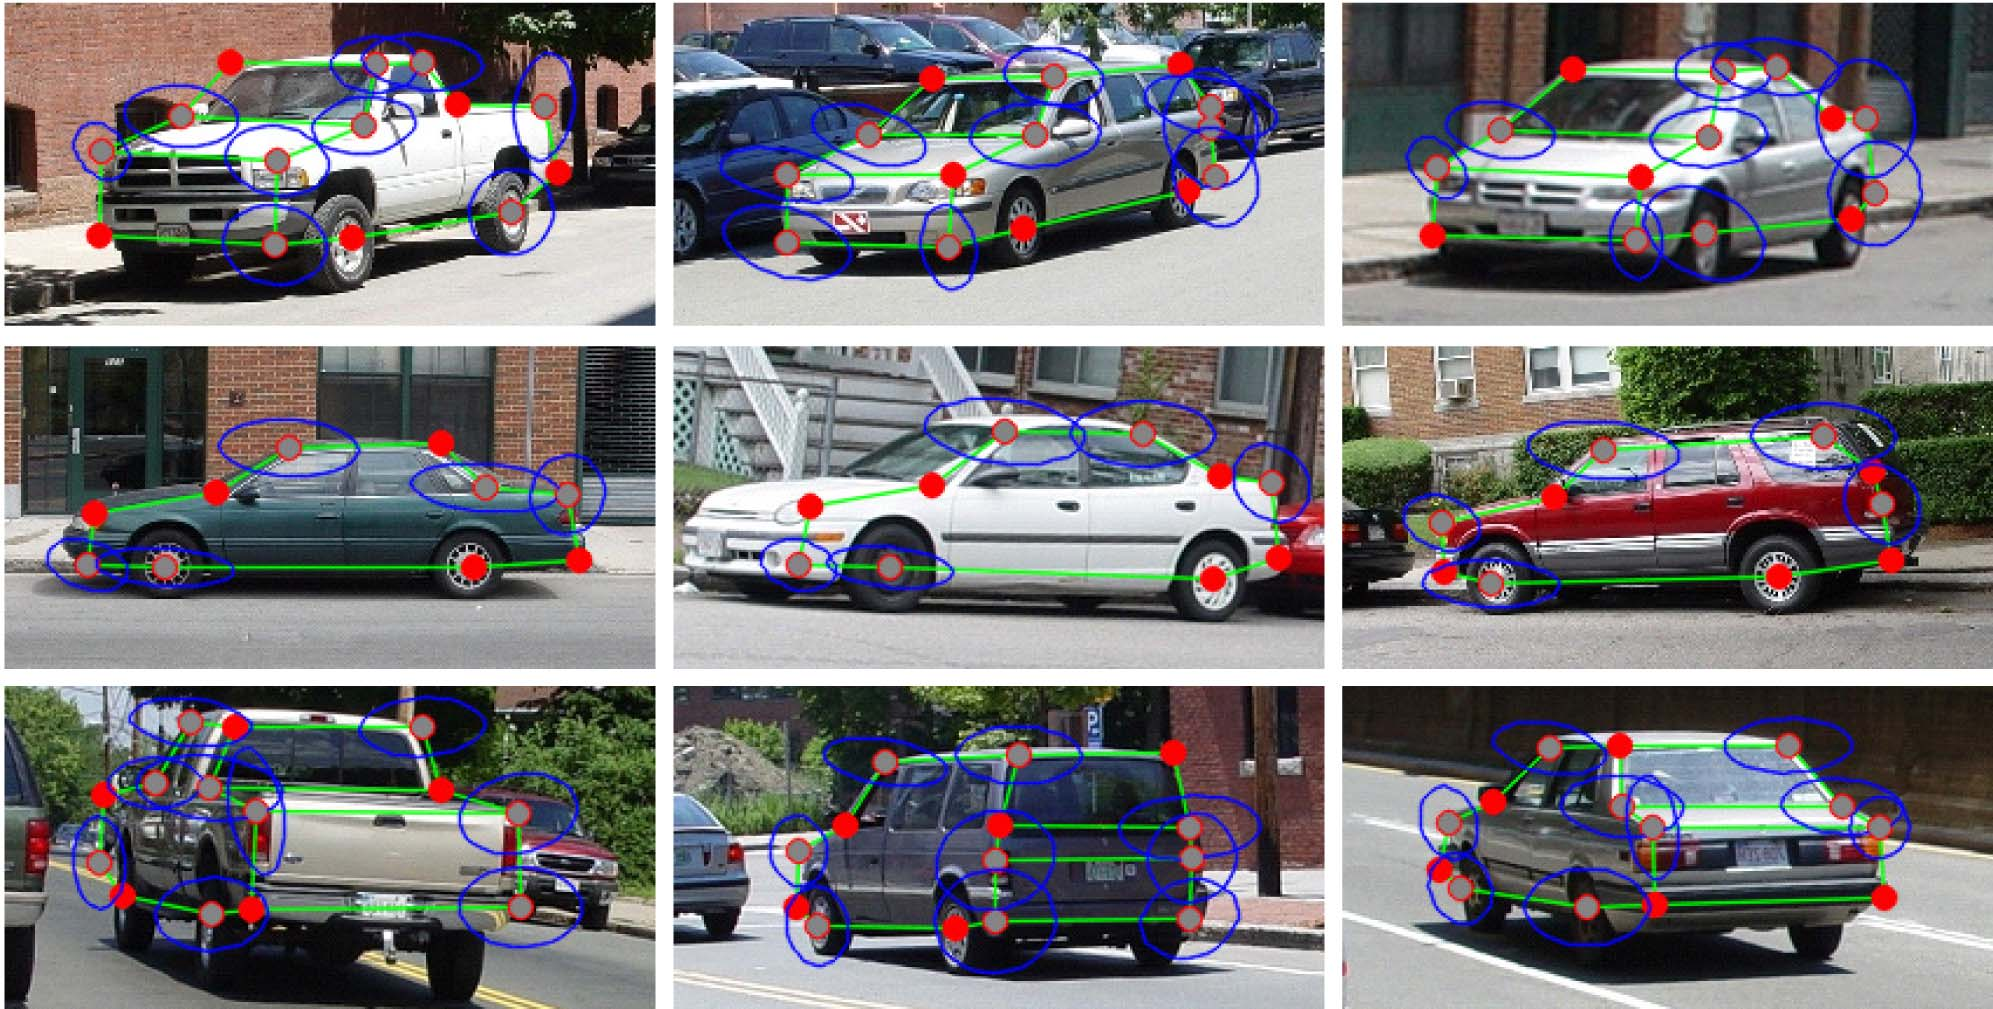
\includegraphics[width=10cm]{images/shape-alignment.jpg}
        \end{figure}
      }
  \end{itemize}
\end{frame}


\section{\hspace{-3mm}Geometric Consistency}
\begin{frame}
  \sectionpage
\end{frame}

\begin{frame}{Geometric consistency}
  \vspace{1mm}
  \textbf{Core Idea}: Leverage invariant properties of transformation model rather than data similarity. If transformation model has an invariant involving a set of points, associations mapping them must preserve that invariant.

  \onslide<2, 3>{
    \only<2>{
      \begin{block}{Point-cloud registration}
        Knowing that Euclidean transformation preserves length, we call \( u = (a, a^\prime) \) and \( v = (b, b^\prime) \) consistent if length of $ab$ is equal to $a^\prime b^\prime$.
      \end{block}


      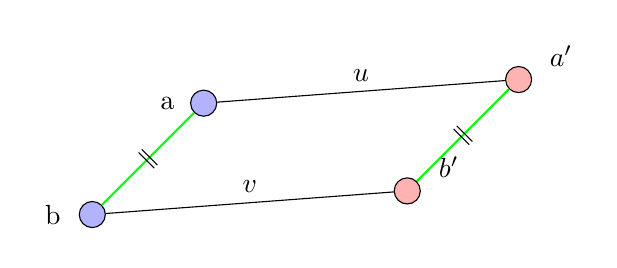
\begin{tikzpicture}[>=stealth, node distance=2cm]
        \tikzstyle{every node}=[circle, draw, fill=blue!30]

        % Nodes
        \node[label=left:a] (a) {};
        \node[label=left:b] (b) [below left of=a] {};

        \tikzstyle{every node}=[circle, minimum size=3mm, draw, fill=red!30, yshift=3mm]

        % Left Nodes
        \node[label=right:$a^\prime$] (a') [right of=a, xshift=2cm] {};
        \node[label=right:$b^\prime$] (b') [right of=b, xshift=2cm] {};

        % Edges
        \tikzstyle{edge} = [draw, thin]
        \tikzstyle{every node}=[]

        \draw[edge] (a) -- node[above, midway] {$u$} (a');
        \draw[edge] (b) -- node[above, midway] {$v$} (b');

        % mark these edge to be equal
        \draw[edge, green, thick] (a) -- (b);
        \draw[edge, green, thick] (a') -- (b');

        \tkzMarkSegment[pos=.5,mark=||](a, b)
        \tkzMarkSegment[pos=.5,mark=||](a', b')

      \end{tikzpicture}
    }


    \begin{block}<3->{Noisy data}
      In noisy-data a \textbf{measure of consistency} is used (binary threshold or a real function $f: \mathbb{R} \to [0, 1]$).
    \end{block}

    \onslide<3->{
      \begin{center}
        \begin{tikzpicture}[scale=0.45]
          \begin{axis}[
              axis lines = middle,
              xlabel = $x$,
              xlabel style={at=(current axis.right of origin), anchor=west},
              ylabel style={at=(current axis.above origin), anchor=south},
              xticklabels={,,},
              yticklabels={,,},
              ymin=0, ymax=1,
              xmin=-2.5, xmax=2.5,
              x=2.2cm,
              every axis x label/.style={at={(ticklabel* cs:1)}, above right,},
              every axis y label/.style={at={(ticklabel* cs:1)}, above right,},
              clip=false,
              domain=-2.5:2.5
            ]
            % Add epsilon lines
            \addplot+[mark=none, dashed, black, domain=-1:1] {0};
            \draw[dashed] (axis cs:-1.7,0) -- (axis cs:-1.7,1);
            \draw[dashed] (axis cs:1.7,0) -- (axis cs:1.7,1);

            \node at (axis cs:-1.7,0) [anchor=north] {$-\varepsilon$};
            \node at (axis cs:1.7,0) [anchor=north] {$\varepsilon$};

            % s(x) function is guassian and zero after 2
            \addplot+[mark=none, samples=1000, blue] {exp(-x^2) * (abs(x) < 1.7)};

            \node at (axis cs:0.5,1) [text=blue] {$s(x)$};

            \node at (axis cs:0,-0.1) {$x = \|a - b\| - \|a' - b'\|$};

          \end{axis}
        \end{tikzpicture}
        %
        \begin{tikzpicture}[scale=0.45]
          \begin{axis}[
              axis lines = middle,
              xlabel = $x$,
              xlabel style={at=(current axis.right of origin), anchor=west},
              ylabel style={at=(current axis.above origin), anchor=south},
              xticklabels={,,},
              yticklabels={,,},
              ymin=0, ymax=1,
              xmin=-2.5, xmax=2.5,
              x=2.2cm,
              every axis x label/.style={at={(ticklabel* cs:1)}, above right,},
              every axis y label/.style={at={(ticklabel* cs:1)}, above right,},
              clip=false,
              domain=-2.5:2.5
            ]
            \addplot+[mark=none, dashed, black, domain=-1:1] {0};
            \draw[dashed] (axis cs:-1.7,0) -- (axis cs:-1.7,1);
            \draw[dashed] (axis cs:1.7,0) -- (axis cs:1.7,1);

            \node at (axis cs:-1.7,0) [anchor=north] {$-\varepsilon$};
            \node at (axis cs:1.7,0) [anchor=north] {$\varepsilon$};

            \addplot+[mark=none, samples=1000, red] {abs(x) < 1.7};

            % s(x) function is guassian and zero after 2

            \node at (axis cs:-0.5,1.1) [text=red]{$r(x)$};
            \node at (axis cs:0,-0.1) {$x = \|a - b\| - \|a' - b'\|$};

          \end{axis}
        \end{tikzpicture}
      \end{center}
    }
  }
  \vspace{\stretch{100}}
\end{frame}



\begin{frame}{Consistency Graph}
  \begin{itemize}
    \item <1->A (weighted) undirected Graph
    \item <2->Each node represents an association
    \item <3->If consistency of $u$ and $u^\prime$ is non-zero there is an (weighted) edge between their respective nodes
    \item <3->If source or terminal of two associations are the same, they are not consistent
  \end{itemize}

  \begin{block}{}
    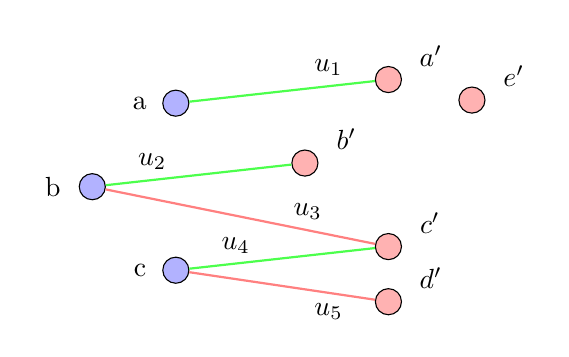
\begin{tikzpicture}[>=stealth, node distance=1.5cm]
      % Define the style for the nodes
      \tikzstyle{every node}=[circle, draw, fill=blue!30]

      % Nodes
      \node[label=left:a] (a) {};
      \node[label=left:b] (b) [below left of=a] {};
      \node[label=left:c] (c) [below right of=b] {};

      % Define the style for the prime nodes
      \tikzstyle{every node}=[circle, minimum size=3mm, draw, fill=red!30, yshift=3mm]

      % Prime Nodes
      \node[label=right:$a^\prime$] (a') [right of=a, xshift=1.2cm] {};
      \node[label=right:$b^\prime$] (b') [right of=b, xshift=1.2cm] {};
      \node[label=right:$c^\prime$] (c') [right of=c, xshift=1.2cm] {};

      \node[label=right:$d^\prime$] (d') [below of=c', yshift=0.5cm] {};
      \node[label=right:$e^\prime$] (e') [below right of=a', yshift=0.5cm] {};

      % Define the style for the edges
      \tikzstyle{edge} = [draw, thick, -]
      \tikzstyle{every node}=[]

      % Edges
      \draw[edge, green!70] (a) -- node[above, near end, black] {$u_1$} (a');
      \draw[edge, green!70] (b) -- node[above, near start, black] {$u_2$} (b');
      \draw[edge, red!50] (b) -- node[above, near end, black] {$u_3$} (c');
      \draw[edge, green!70] (c) -- node[above, near start, black] {$u_4$} (c');
      \draw[edge, red!50] (c) -- node[below, near end, black] {$u_5$} (d');

    \end{tikzpicture}
    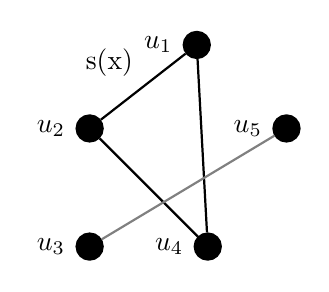
\begin{tikzpicture}[>=stealth, node distance=1.5cm, thick, main/.style = {draw, circle, fill}]

      % Nodes
      \node[main, label=left:$u_1$] (1) {};
      \node[main, label=left:$u_2$, below left of=1, xshift=-3mm] (2) {};
      \node[main, label=left:$u_3$, below of=2] (3) {};
      \node[main, label=left:$u_4$, right of=3] (4) {};
      \node[main, label=left:$u_5$, above of=4, xshift=1cm] (5) {};

      \draw (1) -- (2) node [midway, above left] {s(x)};
      \draw (2) -- (4);
      \draw (1) -- (4);
      \draw[color=black!50] (5) -- (3);

    \end{tikzpicture}
  \end{block}
\end{frame}


\begin{frame}{Affinity Matrix}
  Let $\mathcal{G}$ be consistency graph and $\mathcal{U}$ be the set of associations. Affinity matrix $M$ is defined as:
  \begin{block}{}
    \begin{equation*}
      M = A(\mathcal{G}) + S(\mathcal{U})
    \end{equation*}
  \end{block}

  \begin{itemize}
    \item $A(\mathcal{G})$ is adjacency matrix of $\mathcal{G}$.
    \item $S(\mathcal{U})$ is a diagonal matrix with $S_{ii}$ being the similarity of source and target objects in association $u_i$.
  \end{itemize}


  \begin{alertblock}{No similarity}
    $S(\mathcal{U})$ can be replaced with $\mathcal{I}_n$ if we can't compute similarity.
  \end{alertblock}
\end{frame}


\section{Related Works}
\begin{frame}
  \sectionpage
\end{frame}

\begin{frame}{Related Works}
  \vspace{1mm}
  \begin{itemize}
    \item<1-> Threshold the Consistency Graph
      \only<2,3,4>{
        \begin{block}{MCP}
          If $M$ is binary the \eqref{eq:clipper-main} becomes this

          \begin{equation*}
            \label{eq:clipper-binary}
            \begin{aligned}
               & \underset{\mathbf{u} \in \{0,1\}^n}{\text{maximize}}
               &                                                      & \sum_{i=1}^n u_i                                        \\
               & \text{subject to}
               &                                                      & u_i u_j = 0 \quad \text{if } M(i,j) = 0, \; \forall i,j
            \end{aligned}
          \end{equation*}

          \begin{figure}
            \centering
            \subfloat{
              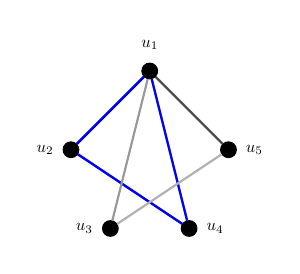
\begin{tikzpicture}[scale=0.5]
                \begin{scope}[thin, every node/.style = {draw, circle, fill, scale=0.6}]
                  \node[label=above:$u_1$] (u1) at (0,2) {};
                  \node[label=left:$u_2$] (u2) at (-2,0) {};
                  \node[label=left:$u_3$] (u3) at (-1,-2) {};
                  \node[label=right:$u_4$] (u4) at (1,-2) {};
                  \node[label=right:$u_5$] (u5) at (2,0) {};
                \end{scope}

                \begin{scope}[every edge/.style={draw=black,thick}]
                  \path (u1) edge[draw=black] (u2);
                  \path (u2) edge[draw=black!70] (u4);
                  \path (u1) edge[draw=black!50] (u4);
                  \only <3> {
                    \path (u1) edge[draw=blue] (u2);
                    \path (u2) edge[draw=blue] (u4);
                    \path (u1) edge[draw=blue] (u4);
                  }

                  \path (u1) edge[draw=black!40] (u3);

                  \path (u1) edge[draw=black!70] (u5);

                  \path (u3) edge[draw=black!30] (u5);
                \end{scope}
              \end{tikzpicture}
            }
            \subfloat{
              \begin{tikzpicture}
                \draw[->, thick] (0, 0) -- (3, 0) node[midway, above] {$e_i > 0$};
                \node (empty) at (0,-1) {};
              \end{tikzpicture}
            }
            \subfloat{
              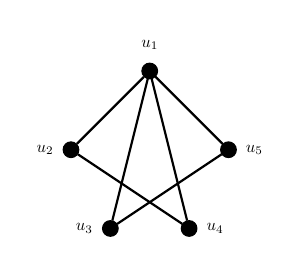
\begin{tikzpicture}[scale=0.5]
                \begin{scope}[thin, every node/.style = {draw, circle, fill, scale=0.6}]
                  \node[label=above:$u_1$] (u1) at (0,2) {};
                  \node[label=left:$u_2$] (u2) at (-2,0) {};
                  \node[label=left:$u_3$] (u3) at (-1,-2) {};
                  \node[label=right:$u_4$] (u4) at (1,-2) {};
                  \node[label=right:$u_5$] (u5) at (2,0) {};
                \end{scope}

                \begin{scope}[every edge/.style={draw=black,thick}]
                  \path (u1) edge (u2);
                  \path (u1) edge (u3);
                  \path (u1) edge (u4);
                  \path (u1) edge (u5);
                  \path (u2) edge (u4);
                  \path (u3) edge (u5);
                \end{scope}
              \end{tikzpicture}
            }
          \end{figure}

          Which is equivalent to solving maximum clique problem.
        \end{block}
      }

    \item<5-> Maximizing sub-graph density
      \only<5,6,7>{
        \begin{block}{Densest Sub-graph}
          By dropping clique constraint we get this

          \begin{equation*}
            \begin{aligned}
              \label{eq:subgraph-maximize}
               & \underset{\mathbf{u} \in \{0,1\}^n\  S = \left.G\right|_u}{\text{maximize}}
               &                                                                             & \frac{\sum_{i \in E(S)} w_i}{\vert S \vert} \onslide<6,7>{= \frac{\mathbf{u}^\top M \mathbf{u}}{\mathbf{u}^\top \mathbf{u}}}
            \end{aligned}
          \end{equation*}

          \only<7>{
            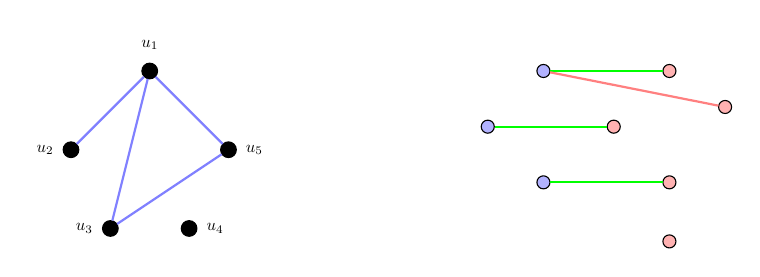
\begin{tikzpicture}[scale=0.5]
              % Define style for the nodes
              \tikzstyle{vertex}=[circle,fill=black,minimum size=8pt,inner sep=0pt]

              % Draw the first graph
              \begin{scope}[thin, every node/.style = {draw, circle, fill, scale=0.6}]
                \node[label=above:$u_1$] (u1) at (0,2) {};
                \node[label=left:$u_2$] (u2) at (-2,0) {};
                \node[label=left:$u_3$] (u3) at (-1,-2) {};
                \node[label=right:$u_4$] (u4) at (1,-2) {};
                \node[label=right:$u_5$] (u5) at (2,0) {};
              \end{scope}

              % Connect vertices with edges
              \draw[thick, blue!50] (u1) -- (u2);
              \draw[thick,blue!50] (u1) -- (u3);
              \draw[thick,blue!50] (u1) -- (u5);
              \draw[thick,blue!50] (u5) -- (u3);

              % Draw the second graph
              \begin{scope}[xshift=10cm, thin]
                \tikzstyle{every node}=[circle,  node distance=2cm, minimum size=3mm, draw, fill=blue!30, scale=0.5]
                % Nodes
                \node(a) at (0, 2) {};
                \node (b) [below left of=a] {};
                \node(c) [below right of=b] {};

                % Define the style for the prime nodes
                \tikzstyle{every node}=[circle, node distance=2cm, minimum size=3mm, draw, fill=red!30, scale=0.5]

                % Prime Nodes
                \node (a') [right of=a, xshift=1.2cm] {};
                \node (b') [right of=b, xshift=1.2cm] {};
                \node (c') [right of=c, xshift=1.2cm] {};
                \node (d') [below of=c', yshift=0.5cm] {};
                \node (e') [below right of=a', yshift=0.5cm] {};

                % Define the style for the edges
                \tikzstyle{edge} = [draw, thick, -]
                \tikzstyle{every node}=[]

                % Edges
                \draw[edge, green] (a) -- (a');
                \draw[edge, green] (b) -- (b');
                \draw[edge, green] (c) -- (c');
                \draw[edge, red!50] (a) -- (e');
              \end{scope}
            \end{tikzpicture}
          }

        \end{block}
      }
  \end{itemize}

  \vspace{\stretch{100}}

\end{frame}


\section{Solution}
\begin{frame}
  \sectionpage
\end{frame}

\begin{frame}{Optimization Formulation}
  Given $M$, affinity matrix, the CLIPPER solves:

  \only<1->{
    \begin{equation}
      \label{eq:clipper-main}
      \begin{aligned}
         & \underset{\mathbf{u} \in \{0,1\}^n}{\text{maximize}}
         &                                                      & \frac{\mathbf{u}^\top M \mathbf{u}}{\mathbf{u}^\top \mathbf{u}} \\
         & \text{subject to}
         &                                                      & u_i u_j = 0 \quad \text{if } M(i,j) = 0, \; \forall i,j
      \end{aligned}
    \end{equation}
  }

  \begin{itemize}
    \item Each element of $u$, indicates that it's respective association is selected
    \item Objective function is normalized sum of weighted edges
    \item Constraints enforce sub-graph to be a clique
  \end{itemize}
\end{frame}

\begin{frame}{Relaxation}
  \vspace{1mm}
  \only<1>{
    \begin{block}{Original Form}
      \begin{equation*}
        \begin{aligned}
           & \underset{\mathbf{u} \in \{0,1\}^n}{\text{maximize}}
           &                                                      & \frac{\mathbf{u}^\top M \mathbf{u}}{\mathbf{u}^\top \mathbf{u}} \\
           & \text{subject to}
           &                                                      & u_i u_j = 0 \quad \text{if } M(i,j) = 0, \; \forall i,j
        \end{aligned}
      \end{equation*}
    \end{block}
  }

  \begin{block}{Relaxed}
    \begin{equation*}
      \begin{aligned}
         & \underset{\mathbf{u} \in \mathbb{R}_+^n}{\text{maximize}}
         &                                                           & \mathbf{u}^\top M_d \mathbf{u} \\
         & \text{subject to}
         &                                                           & \|\mathbf{u}\| \leq 1          \\
      \end{aligned}
    \end{equation*}
  \end{block}

  Where $d$ is increased gradually and $M_d$ defined as
  \begin{equation*}
    M_d(i,j) \vcentcolon= \begin{cases}
      M(i,j) & \text{if } M(i,j) \neq 0 \\
      -d     & \text{if } M(i,j) = 0
    \end{cases}
  \end{equation*}

  \begin{itemize}
    \item<2-> Increasing $d$ would penalizes violation of clique constraint
    \item<3-> For large enough $d$, ($n \leq d$), clique constraints are guaranteed for every optima (local/global)
    \item <4-> For binary graphs, solutions converge to binary values
  \end{itemize}
\end{frame}

\begin{frame}{Solver}
  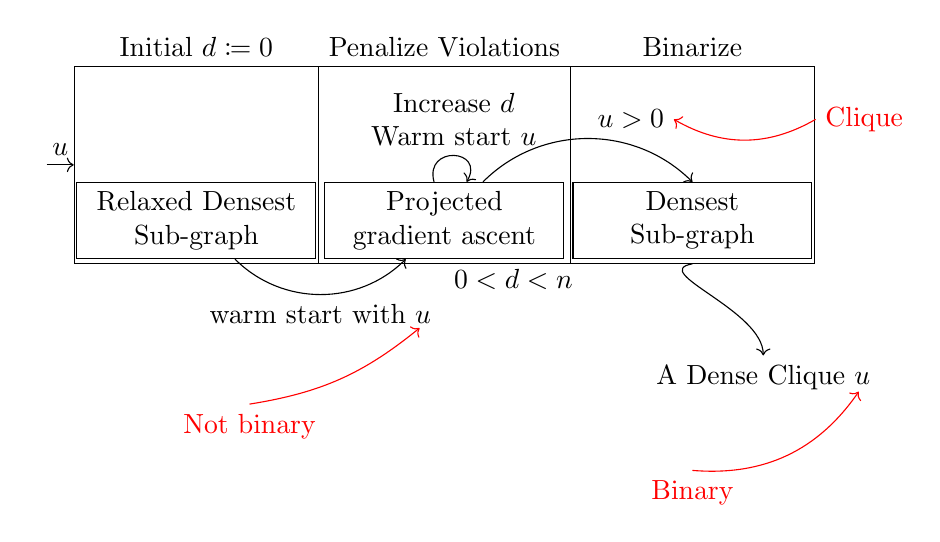
\begin{tikzpicture}[scale=0.45, every node/.style={align=center}]
    \node (start) at (-4.5cm, 0){};


    \onslide<1-> {
      \node[label=above:Initial $d \coloneqq 0$, draw, rectangle, minimum height=2.5cm, minimum width=3.1cm] (d0) at (0, 0) {};
      \draw[->] (start) -- (d0) node[above, midway] {$u$};
    }

    \onslide<2-> {
      \node[rectangle, draw] (densest) [text width=2.8cm] at (0, -1.57) {Relaxed Densest Sub-graph};
    }


    \onslide<3-> {
      \node[label=above:Penalize Violations, draw, rectangle, minimum height=2.5cm, minimum width=3.2cm] (di) at (7, 0) {};
      \node[rectangle, draw] (projected) [text width=2.8cm] at (7, -1.57cm) {Projected gradient ascent};
      \draw[->] (densest) to[bend left=-45] node[below] (init) {warm start with $u$} (projected);
    }

    \onslide<4> {
      \draw[->, red] ($(init.south) - (2cm, 2cm)$) node[below] {Not binary} to [bend right=15] ($(init.east) - (6mm, 4mm)$);
    }

    \onslide<5-> {
      \draw[->] (projected) to [out=105,in=60,looseness=3] node [above, text width=3cm] {Increase $d$\\Warm start $u$} (projected) ;
      \node[anchor=north, below right] () at (projected.south) {$0 < d < n$};
    }

    \onslide<6-> {
      \node[label=above:Binarize, draw, rectangle, minimum height=2.5cm, minimum width=3.1cm] (binary) at (14, 0) {};
    }


    \onslide<7-> {
      \node[rectangle, draw] (graph) [text width=2.8cm] at (14, -1.57cm) {Densest Sub-graph};
      \draw[->] (projected) to[out=45, in=135] node [above right] (ug) {$u > 0$} (graph.north);

      \node (end) at (16, -6) {A Dense Clique $u$};
      \draw[->] (binary.south) to [out=-170,in=90] (end) node [midway, above] {};

    }

    \onslide<8> {
      \draw[->, red] ($(ug.east) + (4cm, 0cm)$) node[right] {Clique} to [bend left=30] (ug.east);
    }

    \onslide<9> {
      \draw[->, red] ($(end.south) - (2cm, 2cm)$) node[below] {Binary} to [bend right=30] ($(end.east) - (6mm, 4mm)$);
    }

  \end{tikzpicture}
\end{frame}

\section{Results}
\begin{frame}
  \sectionpage
\end{frame}


\begin{frame}{Different Outliers}
  \begin{figure}
    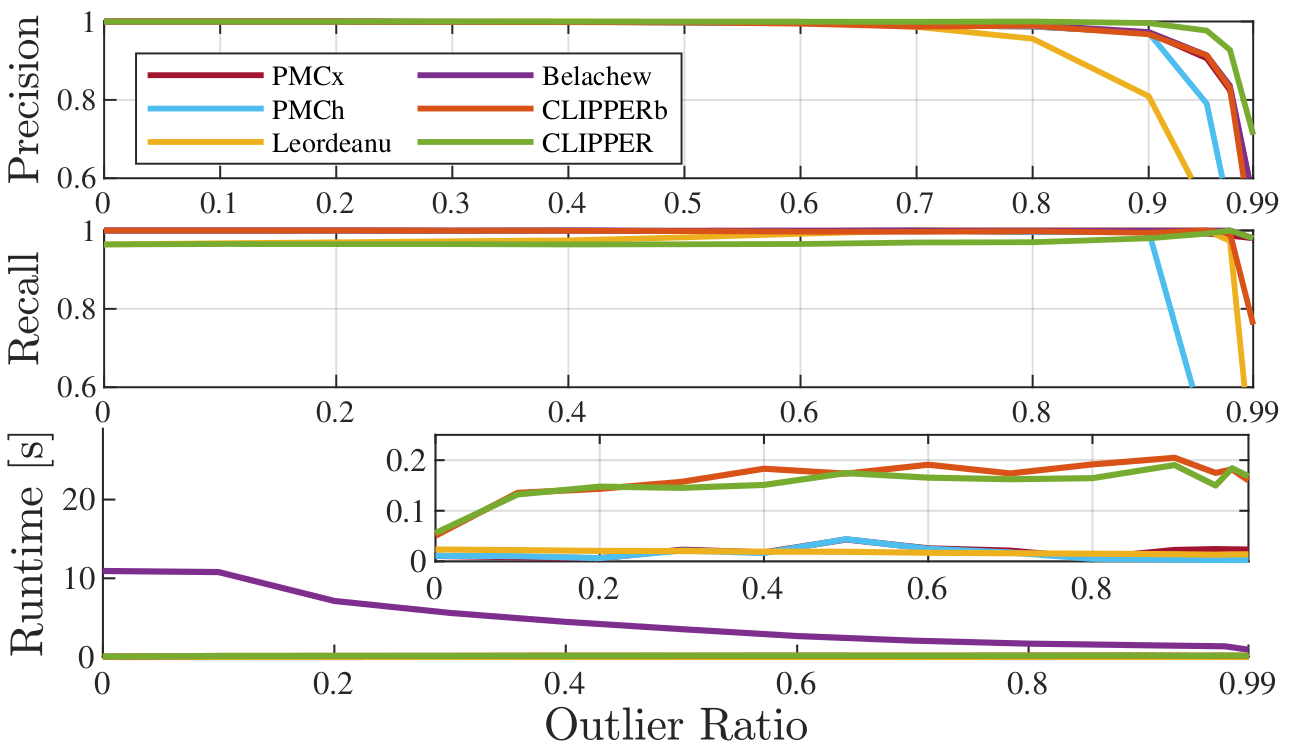
\includegraphics[width=11cm]{images/results-all.png}
  \end{figure}
\end{frame}

\begin{frame}{Different Association Number}
  \begin{figure}
    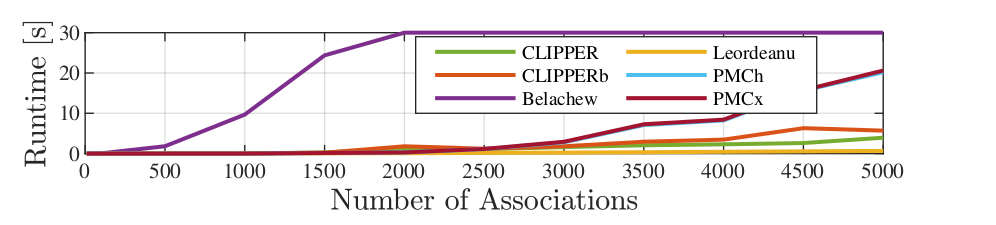
\includegraphics[width=11cm]{images/results-runtime-assoc.png}
  \end{figure}

\end{frame}

\section{Future Work}
\begin{frame}
  \sectionpage
\end{frame}

\begin{frame}{Future Work}
  \begin{itemize}
    \item<1-> In the absence of putative associations runtime grows faster than expected
    \item<2-> Exploring more on transformation that their invariant involve more than two objects
    \item<3-> Structured noise analysis, for example in distortion correction 
    \onslide<3>{
    \begin{figure}
    \centering
    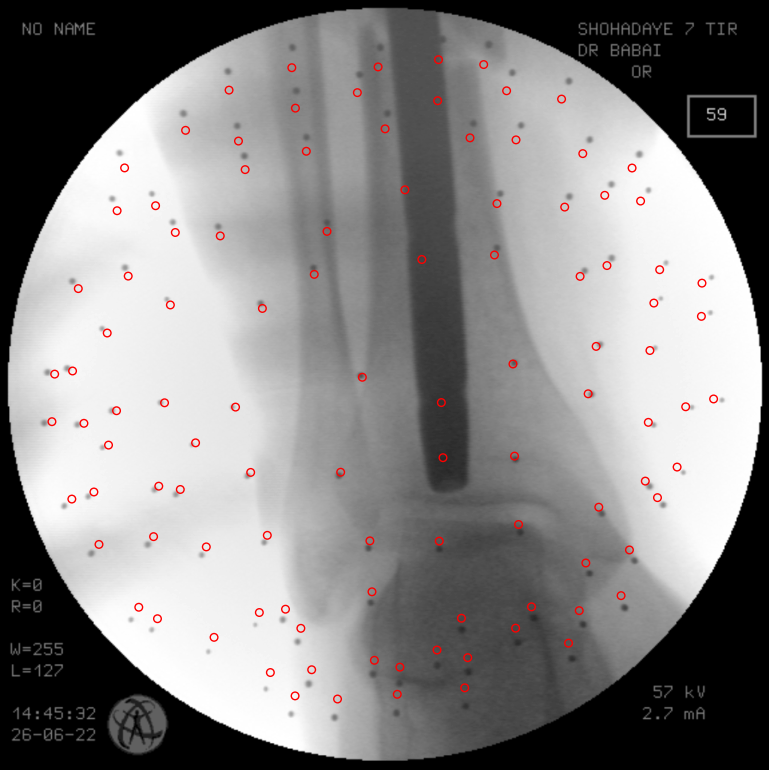
\includegraphics[width=4cm]{images/59-final.png}
    \end{figure}
}
  \end{itemize}
\end{frame}



\begin{frame}{}
  \begin{center}
    \Huge No Questions?\\[2cm]

    \huge Thanks, I'm outta here
  \end{center}
\end{frame}

\end{document}